\section{Pátý týden}

\subsection{Kužel přípustných směrů}
Nechť $M \subseteq \R^n$ a $x \in M$.
\begin{itemize}
    \item Vektor $d \in \R^n$ se nazve přípustný směr množiny $M$ v bodě $x$, jestliže existuje $\delta > 0$ tak, že pro
    každé $\alpha \in (0, \delta]$ je $x + \alpha d \in M$.
    \item Množina $\F(M; x)$ všech přípustných směrů množiny $M$ v bodě $x$ se nazývá kužel přípustných směrů množiny
    $M$ v bodě $x$.
\end{itemize}
$\F(M; x) \not = \emptyset$.\\
Je-li $x \in \Int(M)$, pak $\F(M; x) = \R^n$.\\
Je-li $M$ konečná (neprázdná), pak $\F(M;x) = \bc{0}$ pro každé $x \in M$.

\subsection{Přípustné směry poklesu}
Mějme
\begin{enumerate}[(a)]
    \item Je-li $M = S(0; 1)$, pak $\F(M;x) = \bc{0}$ pro každé $x \in M$.
    \item Je-li $C = B(0; 1)$ a $\hat x = (1, 0)^T$, pak
    \[
        F(C; \hat x) = \bc{
            \begin{bmatrix}
                d_1 \\
                d_2
            \end{bmatrix} \in \R^2 \, \middle| \, d_1 < 0
        } \cup \bc{
            \begin{bmatrix}
                0 \\
                0
            \end{bmatrix}
        }
    \]
\end{enumerate}
(a) $M = S(0; 1) = \bc{x \in \R^2 \mid \| x\| = 1}$

Úvaha: Polopřímka z bodu $(1,0)$ projde maximálně $2 \times$ skrz kružnici.
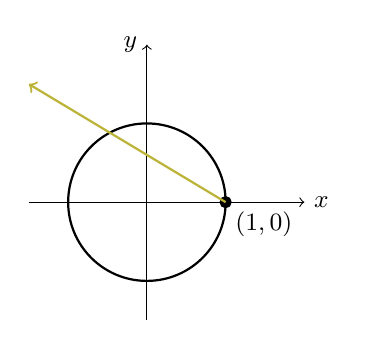
\begin{tikzpicture}
    \draw[thick] (0,0) circle(1);

    \draw[->] (-1.5,0) -- (2,0) node[right] {\small $x$};
    \draw[->] (0,-1.5) -- (0,2) node[left] {\small $y$};

    \filldraw (1,0) circle(2pt) node[below right] {\small $(1,0)$};

    \draw[thick,->, black!30!yellow] (1,0) -- (-1.5,1.5);
\end{tikzpicture}

Ať $d \not = 0 \in \R^2$
\[
    1 = \| x + \alpha d\|^2 = \langle x + \alpha d , x + \alpha d\rangle = \underbrace{\| x\|^2}_{1} + 2 \alpha
    \langle x, d\rangle + \alpha^2 \|d\|^2
\]
\[
    \rightarrow 0 = \alpha (2 \langle x, d\rangle + \alpha \| d\|^2) \implies \alpha =
    - \frac{2 \langle x,d\rangle}{\|d\|^2} \implies \F(M;x) = \bc{0}
\]

(b) Uvažujme kouli \\
$M = S(0; 1) = \bc{x \in \R^2 \mid \| x\| \leq 1}$; $x =
\begin{bmatrix}
    1 \\
    0
\end{bmatrix}$
\[
    1 \geq \left\|
    \begin{bmatrix}
        1 \\
        0
    \end{bmatrix} + \alpha d\right\|^2 = \left\langle
        \begin{bmatrix}
        1 \\
        0
    \end{bmatrix} + \alpha d ,
    \begin{bmatrix}
        1 \\
        0
    \end{bmatrix} + \alpha d\right\rangle = \underbrace{\left\|
    \begin{bmatrix}
        1 \\
        0
    \end{bmatrix}\right\|^2}_{1} + 2 \alpha
    \left\langle
    \begin{bmatrix}
        1 \\
        0
    \end{bmatrix}, d\right\rangle + \alpha^2 \|d\|^2
\]
\[
    \rightarrow 0 \geq \alpha (2 d_1 + \alpha \| d\|^2) \implies \alpha =
    - \frac{2 d_1}{\|d\|^2} \implies \F\left(M;
    \begin{bmatrix}
        1 \\
        0
    \end{bmatrix}\right) = \bc{
    \begin{bmatrix}
        d_1 \\
        d_2
    \end{bmatrix} \in \R^2 \, \middle| \, d_1 < 0
    }.
\]

\subsection{Kužel směrů poklesu}
Nechť $D \subseteq \R^n$, $x \in D$ a $f : D \rightarrow \R$.
\begin{itemize}
    \item Vektor $d \in \R^n$ se nazve směr poklesu funkce $f$ v bodě $x$, jestliže existuje $\delta >0$ tak, že pro
    každé $\alpha \in (0, \delta]$ je $f(x + \alpha d) < f(x)$.
    \item Množina $\D(f; x)$ všech směrů poklesu funkce $f$ v bodě $x$ se nazývá kužel směrů poklesu funkce $f$ v bodě
    $x$.
\end{itemize}
Definice implicitně obsahuje podmínku $[x, x+\delta d] \subseteq D$.

\subsection{Nutná geometrická podmínka lokálního extrému}
Jestliže $x$ je bod lokálního minima funkce $f : D \subseteq \R^n \rightarrow \R$ na $M \subseteq D$, pak
$\F(M; x) \cap D(f;x) = \emptyset$.

Důkaz. Sporem. \\
Ať ne, tj. existuje $d \in \F(M, x) \cap D(f, x)$.\\
Pak: $f (x + \alpha d) < f(x)$ a $x + \alpha d \in M$ pro všechna $\alpha > 0$ dostatečně malá.\\
Tedy spor s tím, že $x$ je bod lokálního minima $f$ na $M$. $\qed$

\subsection{Silný směr poklesu - linearisace směru poklesu}
Nechť $\Omega \subseteq \R^n$ je otevřená množina, $x \in \Omega$ a $f \in C^{1}(\Omega)$.
\begin{itemize}
    \item Vektor $d \in \R^n$ se nazve silný směr poklesu funkce $f$ v bodě $x$, jestliže $\langle \nabla f(x), d\rangle < 0$.
    \item Množina $\D_0(f; x)$ všech silných směrů poklesu funkce $f$ v bodě $x$ se nazývá kužel silných směrů poklesu
    funkce $f$ v bodě $x$.
\end{itemize}
Kužel $\D_0(f; x)$ je množina všech řešení lineární nerovnice \[\langle \nabla f(x), d\rangle < 0.\]
$\D_0(f;x)$ je konvexní kužel.

\subsection{Tvrzení o souvislosti přípustných směrů poklesu a jejich linearisaci}
Nechť $\Omega \subseteq \R^n$ je otevřená množina, $x \in \Omega$ a $f \in C^1(\Omega)$. Potom platí:
\begin{enumerate}[(a)]
    \item Je-li $d \in \D(f; x)$, potom $\langle \nabla f(x), d\rangle \leq 0$.
    \item $\D_0(f;x) \subseteq \D(f;x)$ (tj. jestliže $\langle \nabla f(x), d\rangle < 0$, pak $d \in \D(f;x)$).
\end{enumerate}
Důkaz.\\
(a) Ať $d \in D(f;x)$.
\[
    \frac{f(x + \alpha d) - f(x)}{\alpha} < 0 \text{ pro } \alpha > 0 \text{ dostatečně malé.}
\]
\[
    \implies \underbrace{\lim_{x\rightarrow 0^+ } \frac{f(x+\alpha d - f(x))}{\alpha}}_{= \langle \nabla f(x), d\rangle}
    \leq 0 \qed
\]
\newpage
(b) Ať $\alpha > 0$.
\[
    f(x+\alpha d) = f(x) + \alpha \langle \nabla f(x), d\rangle + \alpha \| d\|
    \overbrace{\omega (\alpha d)}^{\text{zbytek}}
\]
\[
    \frac{f(x+\alpha d) - f(x)}{\alpha} = \underbrace{\langle \nabla f(x), d\rangle + \| d\| \omega (\alpha d)}_{
    \substack{\rightarrow \langle \nabla f(x), d\rangle \text{ pro } \alpha \rightarrow 0^+ \\ \text{a navíc }
    \langle\nabla f(x), d \rangle < 0}} \implies \frac{f(x + \alpha d) - f(x)}{\alpha} < 0
    \text{ pro všechna } \alpha < 0 \text{ dostatečně malá.}
\]

\subsection{Fermatova věta - nutná podmínka optimality}
Nechť $\Omega \subseteq \R^n$ je otevřená množina, $M \subseteq \Omega$ a $\hat x \in M$ je bodem lokálního minima
funkce $f \in C^1(\Omega)$ na $M$. Potom platí:
\begin{enumerate}[(a)]
    \item $\F(M; \hat x) \cap \D_0(f; \hat x) = \emptyset$ (tj. $\langle \nabla f(\hat x), d\rangle \geq 0$ pro všechny
    $d \in \F(M; \hat x)$).
    \item Jestliže $\hat x \in \Int(M)$, pak $\nabla f(\hat x) = 0$.
\end{enumerate}
Důkaz.\\
(a) Víme, že $\F(M; \hat x) \cap \D(f; \hat x) = \emptyset$.\\ \label{fermatA}
Pak:
\[
    \D_0 (f, \hat x) \subseteq D(f, \hat x) \implies \F(M; \hat x) \cap \D_0(f, \hat x) = \emptyset. \qed
\]
(Tj. $\langle \nabla f(\hat x), d\rangle \geq 0 \quad \forall d \in \F(M, \hat x)$)

(b)
\[
    \hat x \in \Int(M) \implies \F(M; \hat x) = \R^n \overset{\hyperref[fermatA]{(a)}}{\implies}
    \langle \nabla f(\hat x), d\rangle \geq 0 \quad \forall d \in \R^n
\]
Ať $d = - \nabla f (\hat x)$.
\[
    - \| \nabla f(\hat x)\|^2 \geq 0 \implies \nabla f(\hat x) = 0. \qed
\]

\subsection{Věta o nutných a postačujících podmínkách pro konvexní úlohu}\label{nutnePostacujiciKonv}
Nechť $\Omega \subseteq \R^n$ je otevřená množina, $f \in C^1 (\Omega)$ je konvexní na $C \subseteq \Omega$ a
$\hat x \in C$. Potom platí:
\begin{enumerate}[(a)]
    \item $\hat x \in \argmin_{x \in C} f(x)$ právě tehdy, když $\F(C; \hat x) \cap \D_0(f; \hat x) = \emptyset$.
    \item Předpokládejme, že $\hat x \in \Int(C)$. Pak $\hat x \in \argmin_{x \in C}f(x)$ právě tehdy, když
    $\nabla f(\hat x) = 0$.
\end{enumerate}
Důkaz.

(a)\\
\enquote{$\Rightarrow$}: Víme. Když máme bod minima, je určitě bodem lokálního minima $\implies$ průnik je prázdný.\\
\enquote{$\Leftarrow$}: Sporem.\\
Ať existuje $y \in C : \overbrace{f(y) < f(\hat x)}^{f(y) - f(\hat x) < 0}$.\\
Ať $d = y - \hat x (\not = 0) \in \F(C, \hat x)$.\\
Cíl: $d \in \F(C, \hat x) \cap \D_0(f, \hat x)$.

\[
    \underbrace{\hat x + \alpha}_{\hat x + \alpha (y- \hat x) = \alpha y + (1-\alpha) \hat x} \hspace*{-11.5mm}d \in C \quad \forall
    \alpha \in [0, 1] \text{ z konvexity } C.
\]
$f$ je konvexní na $C \iff f(\hat x) + \langle \nabla f(\hat x), \overbrace{y - \hat x}^{d}\rangle \leq f(y)$.
$\implies \langle \nabla f(\hat x), d\rangle \leq f(y) - f(\hat x) \underset{\text{z předp.}}{<} 0$.\\
To je ale spor, protože byl předpoklad, že průnik je prázdný. My jsme ale ukázali, že není. $\qed$

(b)\\
\enquote{$\Rightarrow$} Víme.

\enquote{$\Leftarrow$} Ať $\nabla f(\hat x) = 0$.\\
Pak $\langle \nabla f(\hat x), d\rangle = 0 \quad \forall d \in \R^n = \F (C; \hat x)$. Nemáme tedy žádný směr poklesu
$\overset{\hyperref[nutnePostacujiciKonv]{(a)}}{\implies} \hat x \in \argmin_{x \in C} f(x). \qed$

\subsection{Hledání bodu minima}
$f(x, y) = x^2 + 3y^2 - 2xy + x - 2y$

$\nabla^2 f(x, y) =
\begin{bmatrix}
    \phantom{-}2 & -2 \\
    -2 & \phantom{-}6
\end{bmatrix} \dots$ dle Sylvesterova kritéria je positivně definitní. \\
$\implies f $ je nutně (ryze) konvexní.

\[
    0 = \nabla f(x, y) =
    \begin{bmatrix}
        2x-2y + 1 \\
        6y - 2x -2
    \end{bmatrix} \rightarrow
    \begin{matrix}
    \phantom{-}2x - 2y = -1 \\
    -2x + 6y = \phantom{-}2
    \end{matrix} \rightarrow y = \frac{1}{4} \Rightarrow x = -\frac{1}{4}.
\]